\documentclass[conference]{IEEEtran}

\usepackage[pdftex]{graphicx}
% \usepackage{amsmath}
% \usepackage{afterpage}
% \usepackage{wrapfig}
% \usepackage{tabularx}
% \usepackage{subfigure}
\usepackage{caption}
\usepackage{xcolor}
% \usepackage{tabu}
% \usepackage{booktabs}
% \usepackage{multicol}
% \usepackage{hyperref}

\hyphenation{op-tical net-works semi-conduc-tor}

\begin{document}

\title{DQM4HEP : A generic\\Data Quality Monitoring for High Energy Physics}

\author{

\IEEEauthorblockN{R\'emi \'Et\'e}
\IEEEauthorblockA{Univ, Lyon, Universit\'e Lyon 1, \\
CNRS/IN2P3, IPNL 4 rue E Fermi \\
69622, Villeurbanne CEDEX, France\\
Email: rete@ipnl.in2p3.fr}

\and

\IEEEauthorblockN{Antoine Pingault}
\IEEEauthorblockA{Ghent University, Department of Physics \\
and Astronomy Proeftuinstraat 86,\\
B-9000 Gent, Belgium\\
Email: antoine.pingault@ugent.be}

\and

\IEEEauthorblockN{Laurent Mirabito}
\IEEEauthorblockA{Univ, Lyon, Universit\'e Lyon 1, \\
CNRS/IN2P3, IPNL 4 rue E Fermi \\
69622, Villeurbanne CEDEX, France\\
Email: mirabito@ipnl.in2p3.fr}

}

\maketitle

\IEEEpeerreviewmaketitle

\section{Introduction}

With increasingly sophisticated devices, online data quality monitoring is of a significant importance for the detector and operation efficiency. Monitoring data is also a first step to a certification of the reliability of the recorded data for off-line physics analyses. Experiments usually develop their monitoring system on top of their event data model and file format to access and store data. This dependency has the tendency to tie the monitoring system to its dedicated experiment and leads to difficulties to adapt it to others.

With this in mind, a generic online Data Quality Monitoring (DQM) system has been developed without any assumption on the event data model and data type to treat. A dedicated implementation, based on the LCIO~\cite{LCIO} event data model for the Linear Collider collaboration was also developed. This implementation was put to real condition testing using a combined detector setup with the CALICE~\footnote{CAlorimeter for LInear Collider Experiment} Semi-Digital Hadronic CALorimeter (SDHCAL) and Silicon Tungsten Electronic Calorimeter (SiWECal) prototypes during test beam campaigns at CERN\footnote{Conseil Européen pour la Recherche Nucléaire}.

\section{Key points and software architecture}

The framework is designed to be run in separate processes linked to each other by TCP/IP and HTTP protocols respectively using DIM\cite{DIM} and Mongoose\cite{MONGOOSE}. It is strongly based on a plugin system that allows some part of the software to be switched {\color{red}from one to another - switeched on/off, switched protocols, other?}. As a consequence, the data serialization used to send data across the network is encapsulated in plugins, loaded at run-time by the framework.

\begin{figure}[htbp]
  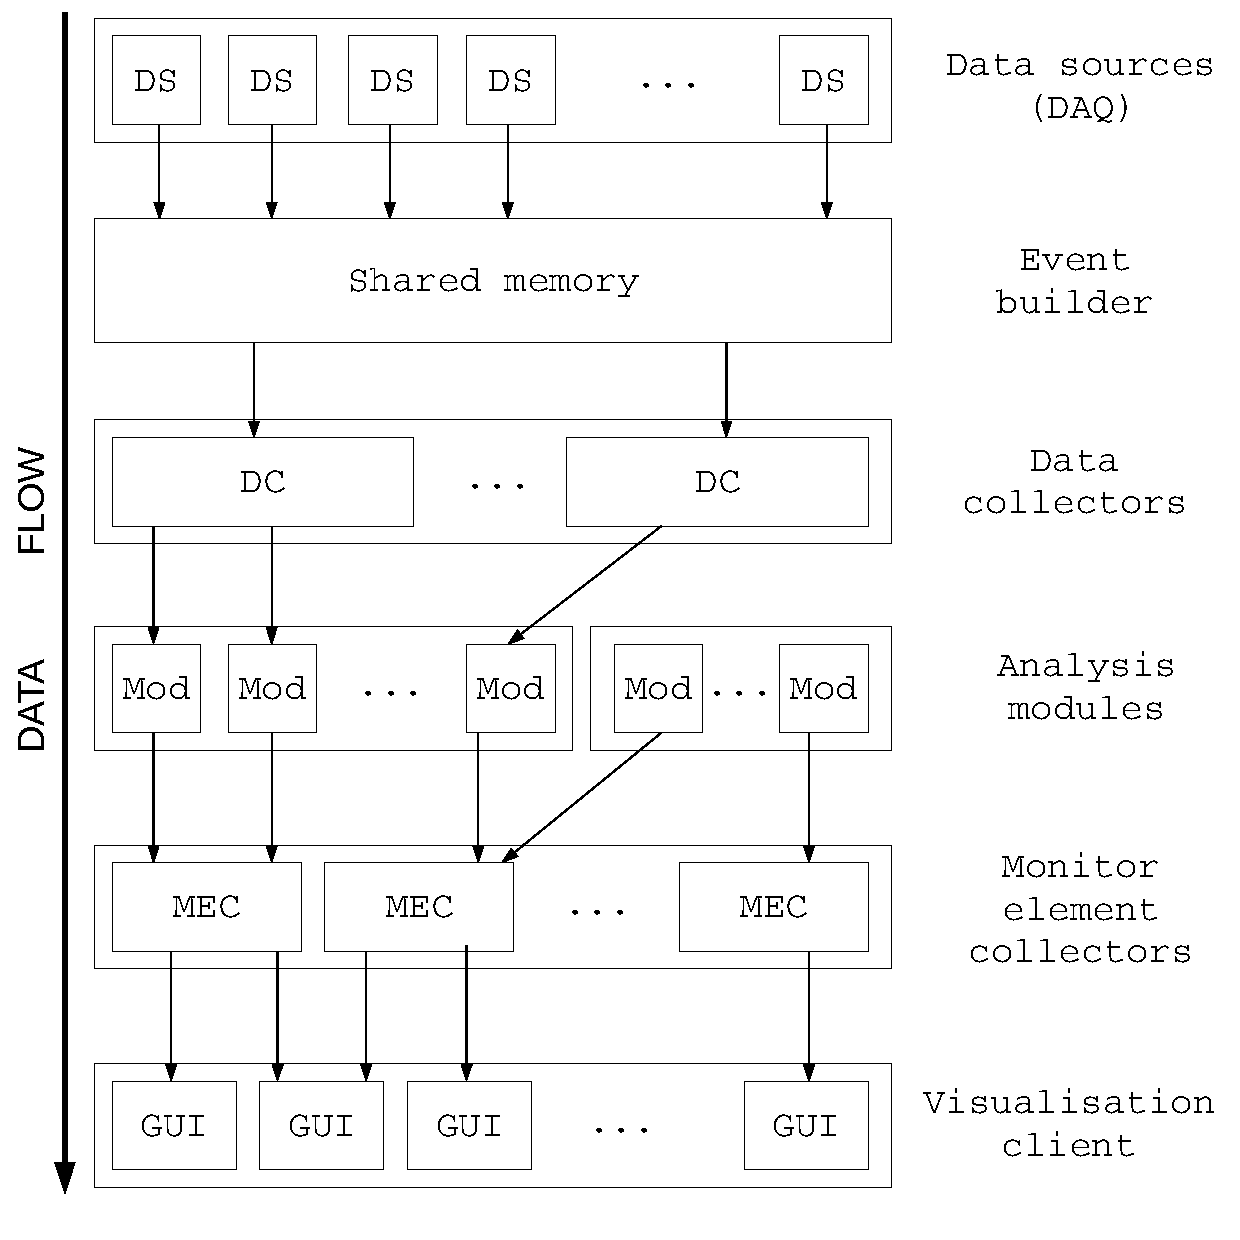
\includegraphics[width=\linewidth]{DQMWorkflow.pdf}
  \caption{\label{DQM_WORKFLOW}The monitoring framework data flow: from data sources to visualization.}
\end{figure}

Fig.~\ref{DQM_WORKFLOW} shows the monitoring framework data flow from incoming data sources to the client visualization computers. An important effort has been put on the creation of a generic interface to the data acquisition system and the development of an event builder. An independent data acquisition (DAQ) process dumps the data sources content in the shared memory (shm) until a given limit in bytes is reached (set by the DAQ). In this way, a slow data treatment by the monitoring will not affect the data taking and writing to disk. Since the data structure is setup dependent, the implementation of the event builder becomes highly specific. The event building is encapsulated in series of \textit{shm processors} that convert data sources buffers into the user data structure. The whole reconstructed event is then serialized, dispatched across the network and stored into one or multiple data collector server applications.

Client interfaces are provided to perform either manual queries of collected data or work in an update mode. When in this mode the data is automatically forwarded from the data collectors to the. Online data analysis developed by the users are also implemented as plugins in the system and steered using configuration files, increasing the modularity of the framework. They use a data collector client interface in update mode to receive and process collected data in an online way.

The main aim of the online data analysis is to reduce the initial amount of data to a few monitorable quantities summarizing its quality and the status of the detection systems. Such quantities have been encapsulated in an unique interface called 'monitor element'. An API is provided for the online analysis module to book and publish frequently these elements across the network. Published monitor elements are in their turn collected by server applications and distributed to visualization clients, again, either on manual query or in update mode.

To visualize monitor elements from the collectors, a graphical user interface has been developed using the Qt\cite{QT} GUI\footnote{Graphical User Interface} toolkit. It can use multiple client interfaces to every available collectors on the network. The user can then display received \textit{monitor elements} in areas organized in tabs. Multiple configurations with different sets of monitor elements can be set-up at once. This allows for a quick overview of all the critical elements and variables needed for the good operation of the experiment.


%%%%%%%%%%%%%%%%%%%%%%%%%%%%%%%%%%%%%%%%%%%%%%%%%%%%%%%%%%%%%%%%%%%
%%%%%%%%%%%%%%%%%%%%%%%%%%%%%%%%%%%%%%%%%%%%%%%%%%%%%%%%%%%%%%%%%%%
\section{Implementation and tests}
In order to test the framework a dedicated implementation has been developed for the CALICE collaboration and its SDHCAL and SiWEcal prototypes. As the LC collaboration {\color{red}must be defined before} has decided to use the LCIO data model for its data taking and storage, an interface to stream data with this specific format has been written. This interface uses in turn the generic generic data streaming interface of the framework (xdrstream). {\color{red}(or is a specific implementation of the generic xdrstream interface?)}

%%%%%%%%%%%%%%%%%%%%%%%%%%%%%%%%%%%%%%%%%%%%%%%%%%%%%%%%%%%%%%%%%%%

As mentioned previously, the CALICE-SDHCAL collaboration has developed a tool to dump online raw data coming from the detectors to a shared memory space as data source buffers. In order to treat these buffers, a specific shm processor plugin needed to be written. It reads the data sent by the DAQ system to the shared memory, then call the online event builder (levbdim) to reconstruct data into the lcio data structure. The reconstructed events are finally wrapped into {\color{red}(serialized as)} generic DQMEvents before being sent over the network to the generic event{\color{red}(data)} collector. Data can then be de-serialized and converted to a format suitable for the online analysis.

The lcio data model contains multiple data format depending on the level of its reconstruction status, and analysis can use any one of them. To overcome this problem, data converters are provided to pass from one lcio data format to the other. This gives the ability to plug off-line analysis, that usually do not take raw events as input, into the monitoring system. The utility being to be able to better asses the overall quality of the incoming data.
The streamer developed for the lcio file format only need files containing lcio formatted data as input, thus the monitoring system can also be tested with off-line data files. In order to keep conditions as close as possible to a real setup, data collectors responsible for forwarding data from the streamer to the analysis modules can be configured to simulate the timing structure of the raw data.


%%%%%%%%%%%%%%%%%%%%%%%%%%%%%%%%%%%%%%%%%%%%%%%%%%%%%%%%%%%%%%%%%%%
For the two week test beam campaign at CERN, specific analysis aimed to the monitoring of the SDHCAL and SiWEcal have also been developed. They come as modules to plug into the framework, and do not depends on each other...{\color{red}But they might? Chain modules with converter for example}. Any modules can be started or stopped, voluntarily or not, at any given time. This implies that even a buggy analysis that would come to crash will not be interfering with the rest of the monitoring{\color{red}Except huge memory leak maybe? =)}. All the modules are configurable through xml files: most of the parameters can be quickly adjusted {\color{red}on the fly}, seconds prior to start the module.

They include a module to monitor the slow control parameters (high and low voltages, pressure, temperature, etc.). As these informations do not come from the DAQ system it is developed as a standalone module that do not run on data coming from data collectors (see right analysis module block in Fig.~\ref{DQM_WORKFLOW}).
One analysis is dedicated to the raw data study and permits the shifters to quickly discover and try to correct for noisy part of the detector. A beam study analysis is available to display metrics about the beam spill such as its length, timing structure, number of acquisition per spill, etc. Some monitor elements from this module can also be used as performances indicators, one practical example would be the number of event treated by the monitoring system versus incoming events coming from the DAQ system.
Other modules are dedicated to efficiency measurement of various parts of the detectors, particle identification or tracking. Specific information using core properties of the detectors are also recorded like the deposited energy (SiWEcal) or number of hits for a given threshold (SDHCAL) for example. Finally event displays modules are also present to visualise particles interactions inside the detectors.

The marlin\cite{MARLIN} framework being widely used inside the LC collaboration for data analysis, an implementation of it is under development and will permit users to directly plug their analysis as it is into the monitoring.

For the test beam campaign combining the two detectors at CERN the following set-up has been successfully deployed:
  \begin{itemize}
  \item Two computers, each one running an event and a monitor element collector and a given set of analysis module.
  \item Multiple monitoring GUIs running on these computers and personal shifters equipment.
  \end{itemize}


\section{Conclusion}
In light of the critical importance of a mean to quickly detect and correct problems in a running experiment as well as the need to insure good and consistent data quality, a new generic framework for Data Quality Monitoring systems has been created. Contrary to most systems available for high energy physics up to now it is not tied to a given experiment set-up. All the tools needed to develop a specific implementation depending on specificities of the experiment, such as data format {\color{red}add something} , are provided within the framework.
In order to put to test this system a dedicated implementation has been developed in parallel for the CALICE SDHCAL and SiWEcal collaborations. The whole system has been successfully used to monitor both prototypes during a two week test beam campaign at CERN. The results are satisfactory and the framework is now in its final stage to being tested within other collaboration

\begin{thebibliography}{1}

% \bibitem{IEEEhowto:kopka}
% H.~Kopka and P.~W. Daly, \emph{A Guide to \LaTeX}, 3rd~ed.\hskip 1em plus
%   0.5em minus 0.4em\relax Harlow, England: Addison-Wesley, 1999.
  
\bibitem{QT}
Qt Company, \emph{\tt http://www.qt.io}, v4.7, 2016.

\bibitem{dim1993distributed}
C. Gaspar et al., \emph{DIM”, International Conference on Computing in High Energy and Nuclear Physics} (Padova,  Italy,
1-11 February 2000)

\bibitem{MONGOOSE}
Michael J Hammel. \emph{Mongoose: an embeddable web server in C}, Linux Journal, 2010(192):2, 2010.

\bibitem{ROOT}
I. Antcheva \textit{et al.}, Comput. Phys. Commun. \textbf{182}, 1384 (2011)

\end{thebibliography}




% 
%   \begin{abstract}
% 
% With increasingly sophisticated devices, online data quality monitoring is of a significant importance for the detector and operation efficiency. Monitoring data is also a first step to a certification of the reliability of the recorded data for offline physics analyses. Experiments usually develop their event data model and file format to access and store their data. This dependency makes the monitoring systems even more specific for each experiment and leads to difficulties to adapt it for other ones. 
% 
% With this in mind, a generic online data quality monitoring system has been developed without any assumption on the event data model and data type to treat. A specific implementation was developed based on the LCIO event data model for the Linear Collider collaboration and used to monitor the data taking of the CALICE SDHCAL and SiWECal prototypes during beam test compaigns at CERN. 
% 
% After introducing the key points of the framework, the software architecture is introduced with the key technical aspects. Details on the specific implementation for the ILC collaboration are presented. Finally, tests on the CALICE SDHCAL and SiWEcal combined detector setup using this implementation are described and used as proof of concept.
% 
% 
%   
%   
%   
% With increasingly sophisticated devices, online data quality monitoring is of a significant importance for the detector and operation efficiency. Monitoring data is also a first step to a certification of the reliability of the recorded data for offline physics analyses. The amount of data to treat in such experiments, becoming larger and larger, makes the monitoring systems more complex. To fastly evaluate data quality and detect anomalies during operation, automated procedures have to be set up. Experiments usually develop their event data model and file format to access and store their data. This dependency makes the monitoring systems even more specific for each experiment and leads to difficulties to adapt it for other ones. \\
% 
% With this in mind, a generic online data quality monitoring system has been developed without any assumption on the event data model and data type to treat. Different applications have been developed and designed to be run in separate processes linked using TPC/IP and HTTP protocols. An important effort has been put on a generic interface to the data acquisition system and the development of an event builder. The framework is strongly based on a plugin system that allows some part of the monitoring system to be switch from one to another. Thus, the data streaming is encapsulated in a plugin, loaded at runtime by the framework. Users online data analysis are also implemented as plugins in the system and steered using configuration files, increasing the modularity of the framework across the different possible experiments. Monitorable quantities have been encapsulated in a unique interface called 'monitor element' that analysis can book and publish frenquently accros the network. Distributed systems have been implemented for detector data and monitor elements in server applications to share available data and reduce the network load per process. \\
% 
% A specific implementation was developed based on the LCIO event data model for the Linear Collider collaboration and used to monitor the data taking of the CALICE SDHCAL prototype during beam test compaigns at CERN in real condition. A combined detector setup with the SiWECal prototype also maked the possibility to test the monitoring software with multiple data sources. \\
% 
% After introducing the key points of the framework, the software architecture is introduced with the key technical aspects. Details on the specific implementation for the ILC collaboration are presented. Finally, tests on the CALICE SDHCAL and SiWEcal combined detector setup using this implementation are described and used as proof of concept.
% 
%   \end{abstract}

  
\end{document}
